\chapter{The Standard Model of Particle Physics}

Ever since Democritus' philosophy of atomism, one of the driving desires behind mankind's advancements in the fields of natural science has been to reduce reality to its basic components.

[...], this chapter explores the theoretical framework for the rest of thesis, introducing key concepts such as \textit{spin}, \textit{helicity} and the importance of \textit{angular distributions} of decay products.

\section{Elementary particles}
\begin{figure}[t!]
	\centering
	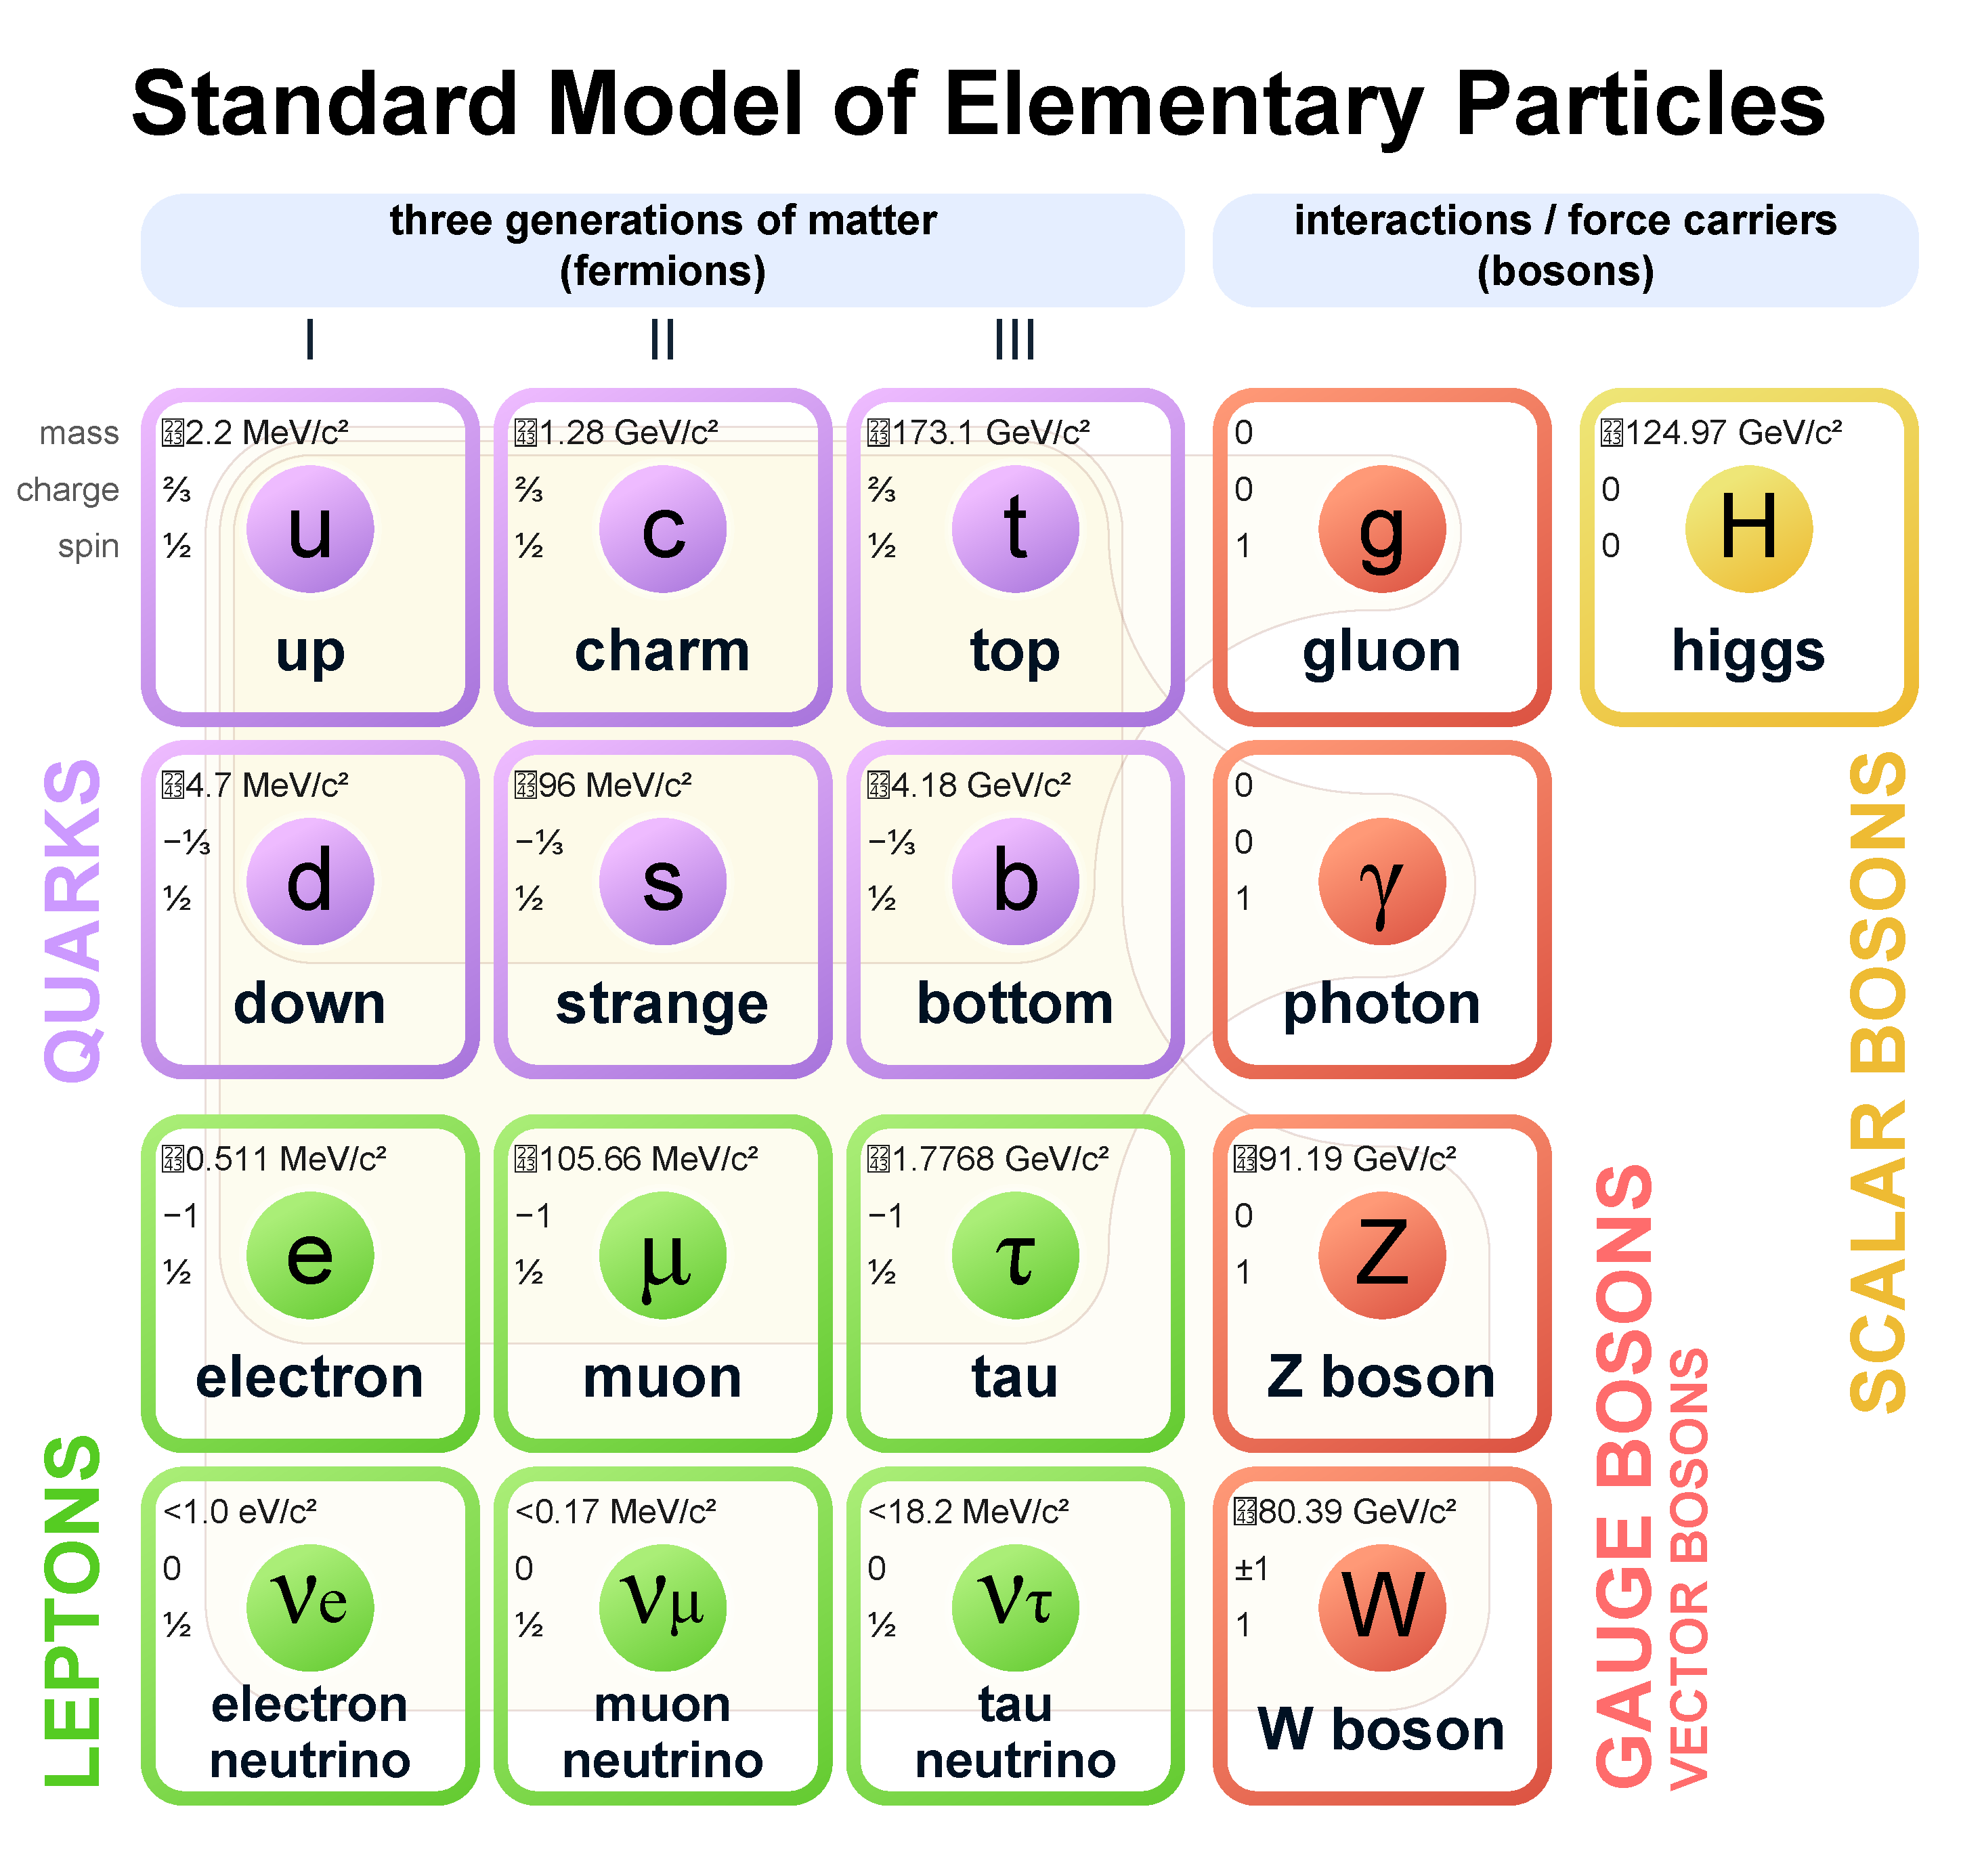
\includegraphics[scale=0.15]{graphics/01-standard_model/Standard_Model_of_Elementary_Particles.pdf}
	\caption[Currently known Standard Model elementary particles.]{The seventeen currently known elementary particles in the Standard Model of Particle Physics. Antiparticles are not depicted.}
	\label{fig:particle_zoo}
\end{figure}

Intuitively, a particle is said to be \textit{elementary} when it displays no substructure that we know of. 
A century of efforts in the fields of nuclear, quantum and high energy physics has whittled down the spectrum of matter to just seventeen unique fundamental particles, colloquially known as the \textit{particle zoo} and depicted in Figure \ref{fig:particle_zoo}.

Each of the ten charged particles is joined by an \textit{antimatter particle} (\textit{antiparticle} for short), a companion of opposite charge identified by the \textit{anti-} prefix, e.g. antimuon for the muon. While often omitted for the sake of brevity, antiparticles are elementary particles in every respect, distinct from their partners and related to them through the transformation of \textit{charge conjugation}.

\subsection{Quarks}
Adroni, mesoni e barioni. QCD. Storia della scoperta.

\subsection{Leptons}

\subsection{Gauge bosons}

\subsection{The Higgs boson}

\section{Spin}
Spin ed EM dipole.

\section{Discrete symmetries}
CPT, violazione di CP.

\section{Helicity formalism}
Il Richman.